\documentclass[sigconf,review,anonymous=false]{acmart}

%% Copyright information
\setcopyright{acmcopyright} % TODO: copyright?
\copyrightyear{2022}
\acmYear{2022}
\acmDOI{10.1145/1122445.1122456} % TODO: DOI?

%% These commands are for a PROCEEDINGS abstract or paper.
\acmConference[Pittsburgh '22]{Pittsburgh '22: NIER - New Ideas and Emerging
Results (ICSE 2022)}{May 21--29, 2022}{Pittsburgh, PA, USA}
\acmBooktitle{Pittsburgh '22: NIER - New Ideas and Emerging Results (ICSE 2022),
May 21--29, 2022, Pittsburgh, PA, USA} \acmISBN{978-1-4503-XXXX-X/18/06}
% TODO: ISBN

%% Packages

% \usepackage[paperwidth=8.50in, paperheight=11in]{geometry} %% option clash
\usepackage[T1]{fontenc}
%\usepackage[latin1]{inputenc}

% \usepackage[protrusion=true,expansion=true]{microtype} %% option clash

% for inline lists
\usepackage[inline]{enumitem}
% for nice internal links
\usepackage{hyperref}

\usepackage{listings}

\begin{document}

\lstset{language=haskell, basicstyle=\scriptsize, breaklines=true,
  showspaces=false, showstringspaces=false, breakatwhitespace=true, texcl=true,
  escapeinside={\%*}{*)}}

\title{When Capturing Knowledge Improves Productivity}

\author{Jacques Carette}
\orcid{0000-0001-8993-9804}
\affiliation{
  \department{Computing and Software}
  \streetaddress{1280 Main Street West}
  \institution{McMaster University}
  \city{Hamilton}
  \state{Ontario}
  \postcode{L8S 4L8}
  \country{Canada}}
\email{carette@mcmaster.ca}

\author{Spencer Smith}
\orcid{0000-0002-0760-0987}
\affiliation{
  \department{Computing and Software}
  \streetaddress{1280 Main Street West}
  \institution{McMaster University}
  \city{Hamilton}
  \state{Ontario}
  \postcode{L8S 4L8}
  \country{Canada}}
\email{smiths@mcmaster.ca}

\author{Jason Balaci}
%\orcid{0000-0002-0760-0987}
\affiliation{
  \department{Computing and Software}
  \streetaddress{1280 Main Street West}
  \institution{McMaster University}
  \city{Hamilton}
  \state{Ontario}
  \postcode{L8S 4L8}
  \country{Canada}}
\email{balacij@mcmaster.ca}

\begin{abstract}
  Current software development is often quite code-centric and aimed at
  short-term deliverables, due to various contextual forces. We're interested in
  contexts where different forces are at play.  \textbf{Well-understood domains}
  and \textbf{long-lived software} provide such an opportunity. By further
  applying generative techniques, aggressive knowledge capture has the real
  potential to greatly increase long-term productivity.

%  Current software development methods are often too short-sighted and too
%  code-centric to be ideally suited to productive long-term development of
%  software (and software families) in well understood domains.  Well understood
%  domains, like scientific and mathematical domains, provide an opportunity for
%  capturing knowledge, which can then be transformed into multiple views in
%  different software artifacts (documentation, code, test cases, build scripts,
%  etc.) within and between projects.  A software
% domain is considered well understood if the domain knowledge can be codified,
% the computational interpretation of the domain knowledge is clear and the
% engineering of code to perform the computations is well understood.  
  Key is to recognize that currently hand-written software artifacts contain
  considerable knowledge duplication. With proper tooling and appropriate
  codification of domain knowledge increasing productivity is feasible. We
  present an example of what this looks like, and the benefits (reuse,
  traceability, change management) thus gained.
%  We present an idealized process that codifies domain knowledge and employs
%  generative techniques to create the required software artifacts.  To be
%  successful, the process requires tool support, which we developed as a set of
%  Domain Specific Languages implemented in Haskell.  The process, along with
%  opportunities for knowledge reuse, traceability and change management, is
%  illustrated via an example of software used to predict the risk of breakage
%  for glass windows subjected to an explosive blast.
\end{abstract}


% Generator:   http://dl.acm.org/ccs.cfm
% TODO: This is a temporary CCSXML and \ccsdesc list
\begin{CCSXML}
<ccs2012>
   <concept>
       <concept_id>10011007.10011006.10011066.10011070</concept_id>
       <concept_desc>Software and its engineering~Application specific development environments</concept_desc>
       <concept_significance>300</concept_significance>
       </concept>
   <concept>
       <concept_id>10011007.10011074.10011075.10011076</concept_id>
       <concept_desc>Software and its engineering~Requirements analysis</concept_desc>
       <concept_significance>300</concept_significance>
       </concept>
   <concept>
       <concept_id>10011007.10011006.10011060.10011690</concept_id>
       <concept_desc>Software and its engineering~Specification languages</concept_desc>
       <concept_significance>300</concept_significance>
       </concept>
   <concept>
       <concept_id>10011007.10011074.10011092.10011782</concept_id>
       <concept_desc>Software and its engineering~Automatic programming</concept_desc>
       <concept_significance>500</concept_significance>
       </concept>
 </ccs2012>
\end{CCSXML}

\ccsdesc[300]{Software and its engineering~Application specific development environments}
\ccsdesc[300]{Software and its engineering~Requirements analysis}
\ccsdesc[300]{Software and its engineering~Specification languages}
\ccsdesc[500]{Software and its engineering~Automatic programming}
%% End of generated code

\keywords{code generation, document generation, knowledge capture,
  software engineering}

% set up math environment
\newtheorem{defn}{Definition}

\maketitle

\section{The Context}
\subsection{``Well understood'' Software?}\label{ch:wellUnderstood}

\begin{defn}
A software domain is \emph{well understood} if
\begin{enumerate}
\item its Domain Knowledge (DK) is codified,
\item the computational interpretation of the DK is clear, and
\item writing code to perform said computations is well understood.
\end{enumerate}
\end{defn}

By \emph{codified}, we mean that the knowledge exists in standard form in a
variety of textbooks. For example, many engineering domains use
ordinary differential equations as models, the quantities of
interest are known, given standard names and standard units. In other words,
standard vocabulary has been established over time and the body of knowledge is
uncontroversial.

We can refine these high level ideas, using the same numbering,
although the refinement should be
understood more holistically.
\begin{enumerate}
\item Models in the DK \emph{can be} written formally.
\item Models in the DK \emph{can be} turned into functional relations by
 existing mathematical steps.
\item Turning these functional relations into code is an understood
 transformation.
\end{enumerate}
Most importantly, the last two parts
deeply involve \emph{choices}: What quantities are considered inputs, outputs
and parameters to make the model functional? What programming language?  What
software architecture data-structures, algorithms, etc.?

In other words,
\emph{well understood} does not imply \emph{choice free}.  Writing a small 
script to move files could just as easily be done in Bash, Python or Haskell.
In all cases, assuming fluency, the author's job is straightforward because
the domain is well understood.

\subsection{Long-lived software?}
For us, long-lived software is software that is expected to be in continuous
use and evolution for $20$ or more years. The main characteristic of
such software is the \emph{expected turnover} of key staff. This means that
all tacit knowledge about the software will be lost over time if it is not
captured.

\subsection{Productivity?}
We adapt the standard definition of productivity, where inputs are labour,
but adjust the outputs to be knowledge and user satisfaction, where user
satisfaction acts as a proxy for effective quality
(see~\cite{SmithAndCarette2020arXiv} for more).
This explicit emphasis on all knowledge produced, rather than just the
operationalizable knowledge (aka code)
implies that human-reusable knowledge, i.e.\ documentation, should also be
greatly valued.

\subsection{Documentation}
Our definition of well understood also applies to \textbf{documentation} aimed
at humans.  Explicitly:
\begin{enumerate}
\item The meaning of the models is understood at a human-pedagogical
level, i.e.\ it is explainable.
\item Combining models is explainable. Thus \emph{transformers}
  %we mentioned before %this is actually the first time transformers are mentioned
  simultaneously operate on mathematical representations
and on explanations. This requires that English descriptions also be
captured in the same manner as the formal-mathematical knowledge.
\item Similarly, the \emph{transformers} that arise from making software
oriented decisions should be captured with a similar mechanism, and also include
English explanations.
\end{enumerate}

We dub these \emph{triform theories}, as a nod to \emph{biform
theories}~\cite{Farmer2007}. We couple 
\begin{enumerate*}
\item an axiomatic description,
\item a computational description, and
\item an English description
\end{enumerate*}
of a concept.


%\subsection{Choices}
%
%Different kinds of choices are embedded in the different kinds of knowledge.
%They can show up simply as \emph{parameters}, for example the acceleration due
%to the gravity constant associated with a planet. They can also shows up as
%different transformers, for example turning $F - m\cdot a = 0$ into $F\left(m,
%a\right) = m\cdot a$, i.e. from a conservation law into a computation.
%For motion computation that same conservation law is often rewritten as
%$a\left(m,F\right) = F/m$ as part of solving $a = \ddot{x}$ to obtain a position
%($x$) as a function of time ($t$). We also get choices of phrasing, which are
%equivalent but may be more adequate in a given context.

\subsection{Softifacts}

Software currently consists of a whole host of artifacts: requirements,
specifications, user manual, unit tests, system tests, usability tests,
build scripts, READMEs, license documents, process documents, as well as
code. We use the word \emph{softifacts} for this collection.

\subsection{Examples of context}

When are these conditions fulfilled? One example is
\emph{research software} in science and engineering. While the results of
running various simulations is entirely new, the underlying models and
how to simulate them are indeed well-known. One particularly long-lived
example is embedded software for space probes (like Pioneer 10).

\section{A New Development Process}\label{ch:process}

Given appropriate infrastructure, what would be an \emph{idealized process}
(akin to Parnas' ideas of faking a rational design process \cite{Parnas1986})
in such a scenario?

\begin{enumerate}
\item\label{it:problem} Have a task to achieve where
\emph{software} can play a central part in the solution.
\item\label{it:understood} The underlying problem domain
is \emph{well understood}.
\item\label{it:probdesc} Describe the problem:
  \begin{enumerate}
  \item Find the base knowledge (theory) in the pre-existing library
    or, failing that, write it if it does not yet exist,
    for instance the naturally occurring known quantities and
    associated constraints.
  \item Assemble the ingredients into a coherent narrative,
  \item Describe the characteristics of a good solution,
  \item Come up with basic examples (to test correctness, intuitions, etc).
  \end{enumerate}
\item\label{it:refine} Describe, by successive refinement transformations, how
the above can be turned into a
deterministic\footnote{A current meta-design choice.}
input-output process.
  \begin{enumerate}
  \item Some refinements will involve \emph{specialization}
    (eg. from $n$-dimensional to $2$-dimensional, assuming no
    friction, etc).  These \emph{choices} and their \emph{rationale} need to be
    documented, as a a crucial part of the solution.  Whether these choices
    are (un)likely to change in the future should be recorded.
  \item Choices tend to be dependent, and thus (partially) ordered.
   \emph{Decisions} frequently enable or reveal downstream choices.
  \end{enumerate}
\item\label{it:tocode} Describe how the process from step
\ref{it:refine} can be turned into code. The same kinds of choice
can occur here.
\item\label{it:recipe} Turn the steps (i.e.\ from items~\ref{it:refine} and
\ref{it:tocode}) into a \emph{recipe}, aka program, that weaves together all the
information into a variety of artifacts (documentation, code, build scripts,
test cases, etc). These can be read, or executed, or \ldots\, as appropriate.
\end{enumerate}

While this last step might appear somewhat magical, it isn't. The whole point of
defining \emph{well understood} is to enable it! A \emph{suitable}
knowledge encoding is key to enable it. This is usually tacit knowledge that
entirely resides in developers' heads.

What is missing is an explicit \emph{information architecture} of each of
the necessary artifact. In other words, what information is necessary to
enable the mechanized generation of each artifact? It turns out that many
of them are quite straightforward.

Often steps~\ref{it:problem} and~\ref{it:probdesc} are skipped; this is
part of the \textbf{tacit knowledge} of a lot
of software.  Our process requires that this knowledge be made explicit,
a fundamental step in \emph{Knowledge Management}~\cite{Dalkir2011}.

% TODO: insert graphical illustration of the funnel from information to
% softifacts.

\section{An Example}\label{ch:example}

We have built the needed infrastructure. It consists of 60KLoc of Haskell
implementing a series of interaction Domain Specific Languages (DSLs) for
knowledge encodings, mathematical expressions, theories, English fragments,
code generation and document generation\footnote{We will provide a link
if the paper is accepted.} A full description would take too much space.
%because of the double blind review process, we can't really cite Drasil here
Instead, we provide an illustrative example.

We will focus on information capture and the artifacts we can generate.
For concreteness, we'll use a single example from our suite: GlassBR, used
to predict the blast risk involved for a glass window.  The requirements
are based on an American Standard Test Method (ASTM) standard
\cite{BeasonEtAl1998}.

The transformation of captured knowledge is illustrated in
Figure~\ref{Fig_DrasilAndChange}. This is read starting from the upper
right box. Each piece of information in this figure has its own
shape and colour (orange-cloud, pink lozenge, etc). It should be immediate
that all pieces of information reappear in multiple places in the generated
artifacts. For example, the name of the software (GlassBR) ends up
appearing more than 80 times in the generated softifacts (in the folder
structure, requirements, README, Makefile and source code). Changing this
name would traditionally be extremely difficult; we can achiece this by
modifying a single place, and regenerating.

The first box shows the directory structure of the currently generated
softifacts; continuing clockwise, we see examples of Makefiles for
the Java and Python versions, parts of the fully documented, 
generated code for the main computation in those languages, user
instructions for running the code, and the processed \LaTeX for the
requirements.

The name GlassBR is probably the simplest example of what we mean by
\emph{knowledge}: here, the concept ``program name'' is internally defined, and
its \emph{value} is used throughout. A more complex example is that
of the assumption that the ``Load Distribution Factor'' (LDF) is constant
(pink lozenge). If this changes to be an input, the generated software
will have LDF as an input variable.  We also capture design decisions,
such as whether to log all calculations, whether to in-line constants rather
than show them symbolically, etc. The knowledge for GlassBR can also be reused
in different projects.

\begin{figure*}[h]
  \centering
  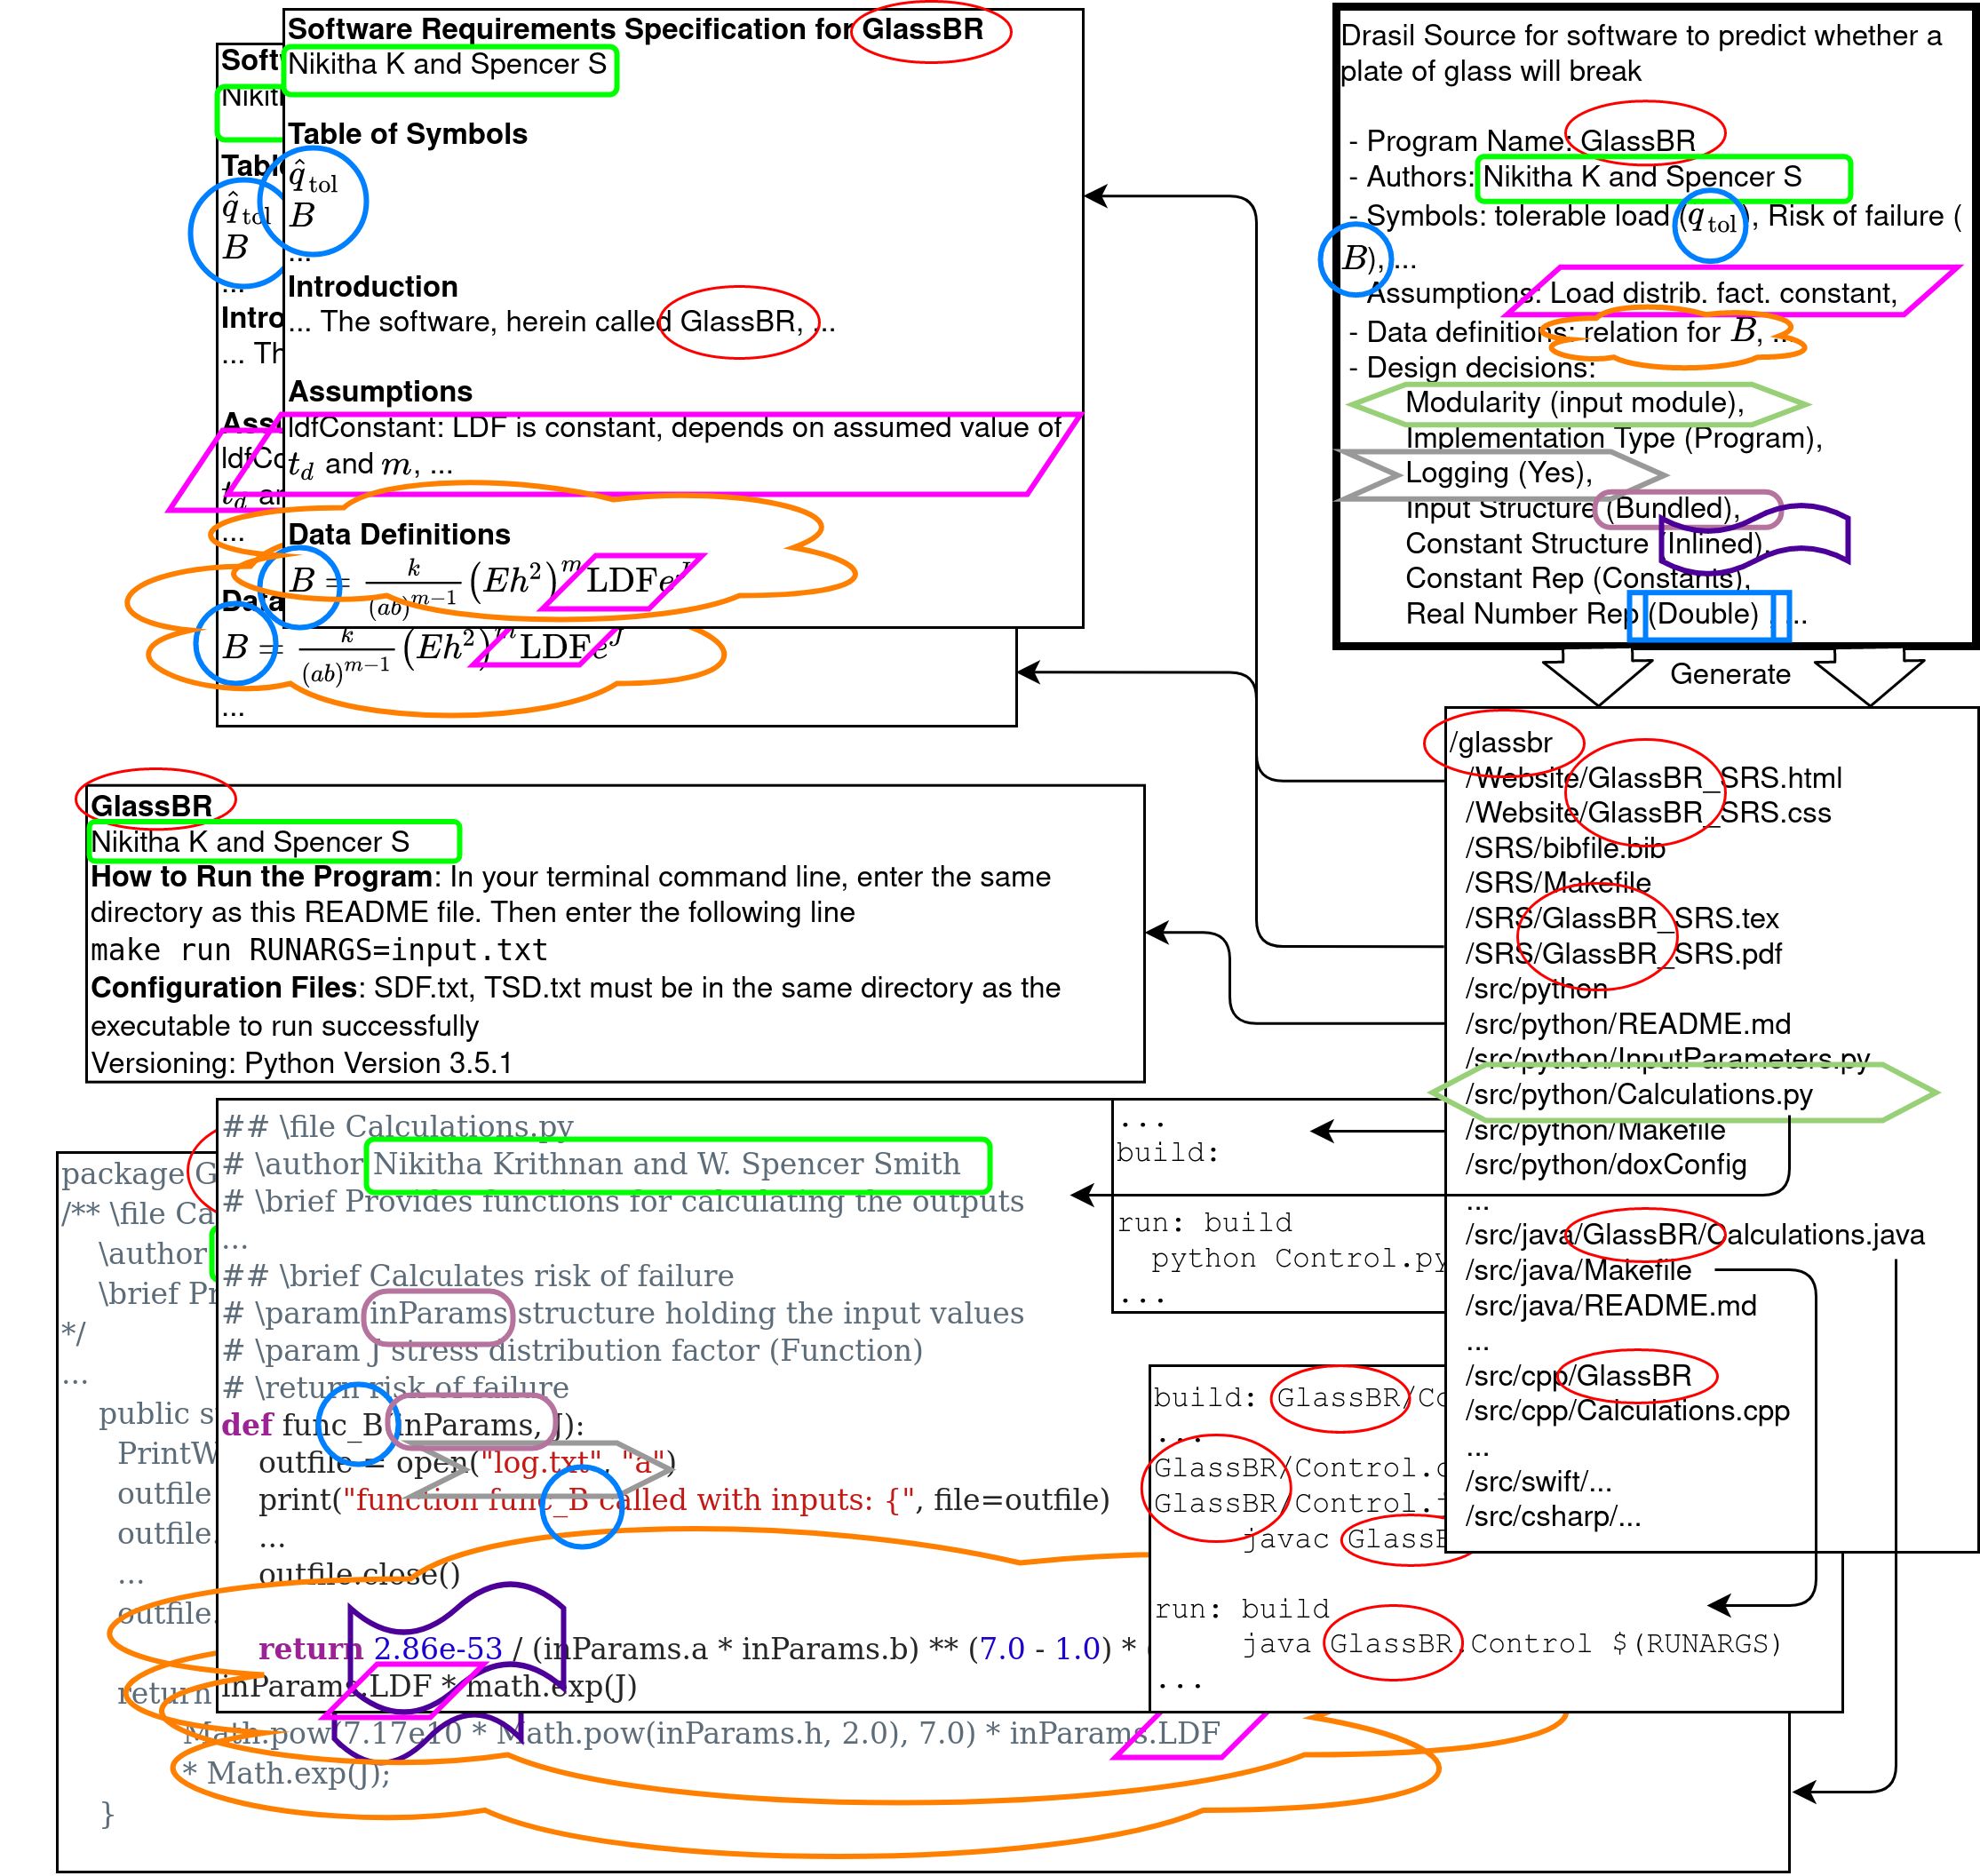
\includegraphics[width=\linewidth]{assets/DrasilSupportsChange-right-portrait-overlapped-ungrouped-11ptFont-squished-v1-300dpi.png}
  \caption{Colors and shapes mapping from captured knowledge to generated
  artifacts.}
  \Description{Colors and shapes mapping from captured knowledge to generated
  artifacts.}
  \label{Fig_DrasilAndChange}
\end{figure*}

We give example encodings\footnote{with some additional abbreviations 
for space.}
corresponding to steps of the process.
\subsection*{Step 3a: Base Knowledge}

\begin{lstlisting}
fullyT, glassTypeFac, heatS, iGlass, lGlass :: CI
fullyT = ci' "fullyT" (np' "fully tempered") "FT" [idglass]
glassTF = ci' "glassTypeFac" (np' "glass type factor") "GTF" [idglass]
heatS = ci' "heatS" (np' "heat strengthened") "HS"[idglass]
iGlass = ci' "iGlass" (np' "insulating glass") "IG"[idglass]
lGlass = ci' "lGlass" (np' "laminated glass") "LG" [idglass]

risk :: DataDefinition
risk = ddE riskQD
 [dRef astm2009, dRefInfo beasonEtAl1998 $ Equation [4, 5],
 dRefInfo campidelli $ Equation [14]] Nothing "riskFun" 
 [aGrtrThanB, hRef, ldfRef, jRef]
 where 
  riskQD = mkQuantDef riskFun riskEq
  riskEq = (sy sflawParamK $/ (mulRe (sy plateLen) (sy plateWidth) $^ (sy sflawParamM $- exactDbl 1))) 
    `mulRe`
        ((sy modElas `mulRe` square (sy minThick)) $^ sy sflawParamM) `mulRe` sy lDurFac `mulRe` exp (sy stressDistFac)
\end{lstlisting}

\subsection*{Step 3b: Coherent Narrative}

As per the requirements template for scientific software~\cite{SmithAndLai2005,
SmithEtAl2007}, we have a goal: ``\textbf{Predict-Glass-Withstands-Explosion}: Analyze and predict whether the glass slab
under consideration will be able to withstand the explosion of a certain degree
which is calculated based on user input.'' The goal statement is generated via:

\begin{lstlisting}
willBreakGS :: ConceptInstance
willBreakGS = cic "willBreakGS" (foldlSent [S "Analyze" `S.and_`
S "predict whether the", phrase glaSlab, S "under consideration will be able",
S "to withstand the", phrase explosion `S.of_` S "a certain", phrase degree_',
S "which is calculated based on", phrase userInput])
"Predict-Glass-Withstands-Explosion" goalStmtDom
\end{lstlisting}

\subsection*{Step 3c: Characteristics of a Good Solution}

We can use the example here that the probability that is calculated has to be
between 0 and 1.

\subsection*{Step 4a: Specialization of Theories}

Theories are specialized via assumptions, like this one: ``\textbf{glassCondition}:
Following astm2009 (pg. 1), this practice does not apply to any form of wired,
patterned, etched, sandblasted, drilled, notched, or grooved glass with surface
and edge treatments that alter the glass strength. (RefBy:
UC:Accommodate-Altered-Glass.)''  This assumptions is generated via:

\begin{lstlisting}
glassConditionDesc :: Sentence
glassConditionDesc = foldlSent [S "Following", complexRef astm2009 (Page [1]) `sC` 
  S "this", phrase practice, S "does not apply to any form of", foldlList Comma Options $ map S ["wired",
  "patterned", "etched", "sandblasted", "drilled", "notched", "grooved glass"], S "with", 
  phrase surface `S.and_` S "edge treatments that alter the glass strength"]
\end{lstlisting}

\subsection*{Step 4b: ?}

We create a closed harmonic system containing all related knowledge (in
particular, the grounded theories), which is as simple as collecting them into a
single system.

\begin{lstlisting}
iMods :: [InstanceModel]
iMods = [pbIsSafe, lrIsSafe]

si :: SystemInformation
si = SI {
_sys = glassBR, _kind = Doc.srs, _authors = [nikitha, spencerSmith],
_purpose = purpDoc glassBR Verbose, _quants = symbolsForTable,
_concepts = [] :: [DefinedQuantityDict], _instModels = iMods,
_datadefs = GB.dataDefs, _configFiles = configFp,
_inputs = inputs, _outputs = outputs,
_defSequence = qDefns, _constraints = constrained,
_constants = constants, _sysinfodb = symbMap,
_usedinfodb = usedDB, refdb = refDB
}
\end{lstlisting}

\subsection*{Step 5}

We make choices about the software representations of the theories:

\begin{lstlisting}
code :: CodeSpec
code = codeSpec fullSI choices allMods

choices :: Choices
choices = defaultChoices {
  lang = [Python, Cpp, CSharp, Java, Swift], modularity = Modular Separated,
  impType = Program, logFile = "log.txt", logging = [LogVar, LogFunc],
  comments = [CommentFunc, CommentClass, CommentMod], doxVerbosity = Quiet,
  dates = Hide, onSfwrConstraint = Exception, onPhysConstraint = Exception,
  inputStructure = Bundled, constStructure = Inline, constRepr = Const,
  auxFiles = [SampleInput "../../datafiles/glassbr/sampleInput.txt", ReadME] 
}
\end{lstlisting}

\subsection*{Step 6}

A final executable program which should take the knowledge discussed above, and
use pre-made printers/generators to generate software artifacts, SRS documents,
etc:

\begin{lstlisting}
main :: IO()
main = do
    setLocaleEncoding utf8
    gen (DocSpec (docChoices SRS [HTML, TeX]) "GlassBR_SRS") srs printSetting
    genCode choices code
    genDot fullSI
    genLog fullSI printSetting
\end{lstlisting}

\section{Concluding Remarks} \label{ch:concluding_remarks}

For well understood domains, building software ought to be a matter of
engineering, based on solid scientific foundations. The ultimate test of ``well
understood'' is being able to teach the domain language to a computer. We have
shown samples of a process and implementation framework for generating all of
the software artifacts for (well understood) software, from the natural
knowledge base of the domain.

We take advantage of inherent knowledge duplication between artifacts in a
project, and between projects, by capturing the knowledge once and providing
means to transform that information into all of the views needed within a given
project.  Developers can realize long-term productivity with documentation and
code that are consistent by construction.

Codifying scientific, engineering and computational knowledge is challenging,
but success will completely transform the development of software, and software
families, in well understood domains. Our process will remove human errors from
generating and maintaining documentation, code, test cases and build
environments, since the mundane details are handled by the generator.  With the
new software tools, we can potentially detect inconsistencies between theory via
inter-theory consistency constraints. Moreover, we can explicitly track the
ramifications of a proposed change.  With the right up-front investment, we can
have sustainable software because stable knowledge is separated from rapidly
changing assumptions and design decisions.

%% Bibliography
\bibliographystyle{ACM-Reference-Format}
\bibliography{References}

\end{document}

% Good quotes:
% \begin{itemize}
% \item metaprograms are just programs
% \item models outside an integrated toolchain are insufficiently useful
% \end{itemize}
